\documentclass{beamer}
\usetheme{Boadilla}
\usepackage{essay-def}
\usepackage{bm}
\usepackage{amsfonts}
\usepackage{amssymb}
\usepackage{amsmath}
\usepackage{amsthm}
\usepackage{comment}
\usepackage{geometry}
\geometry{left=1cm,right=1cm}
    \title[Arcsine Law and Beyond]{Arcsine Law and Time of the Maximum and the Minimum of Stochastic Processes}
\author[H. Yang, J. Zhao (PKU)]{Haoran Yang, Jiaxi Zhao(PKU)}
%\institute[]{joint work with Wuchen Li (UCLA)}
\date{25th September, 2020}
\begin{document}
\par \setlength{\parindent}{2em}

\begin{frame}
\titlepage

\end{frame}


\begin{frame}{Origin: L\'{e}vy's arcsine law}
\par
\begin{figure}[H]
	\centering
  	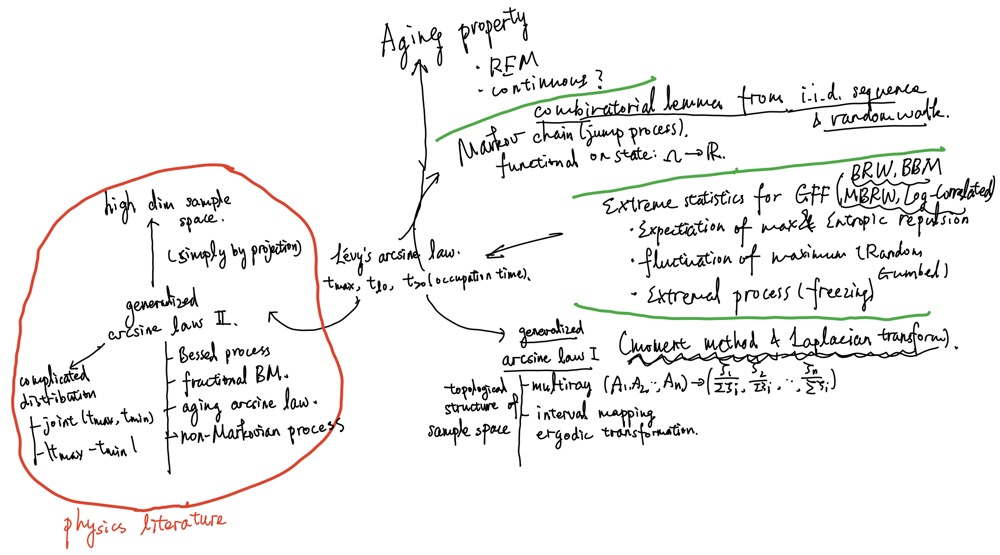
\includegraphics[width=\linewidth]{literature-v2.png}
  	\caption{History}
  	\label{literature}
	\end{figure}
\end{frame}


\begin{frame}{L\'{e}vy's arcsine law}
\par
Denote $X_t$ as standard Brownian motion on $\mbR$. Define three random variables as follows:
\begin{equation}
    \begin{aligned}
        t_{>0} & := \frac{1}{T}\int_0^T \mathbf{1}_{\lb 0, \infty \rpz}\lp X_t \rp \, \mathrm{d} t,    \\
        t_{\max} & := \frac{1}{T}\arg \max_{t \in \lb 0, T \rb} X_t,    \\
        t_{l-0} & := \frac{1}{T}\max_{t \in \lb 0, T \rb} \lbb t \big| X_t = 0 \rbb.    \\
    \end{aligned}
\end{equation}
\end{frame}


\begin{frame}{L\'{e}vy's arcsine law}
\par
\begin{figure}[H]
	\centering
  	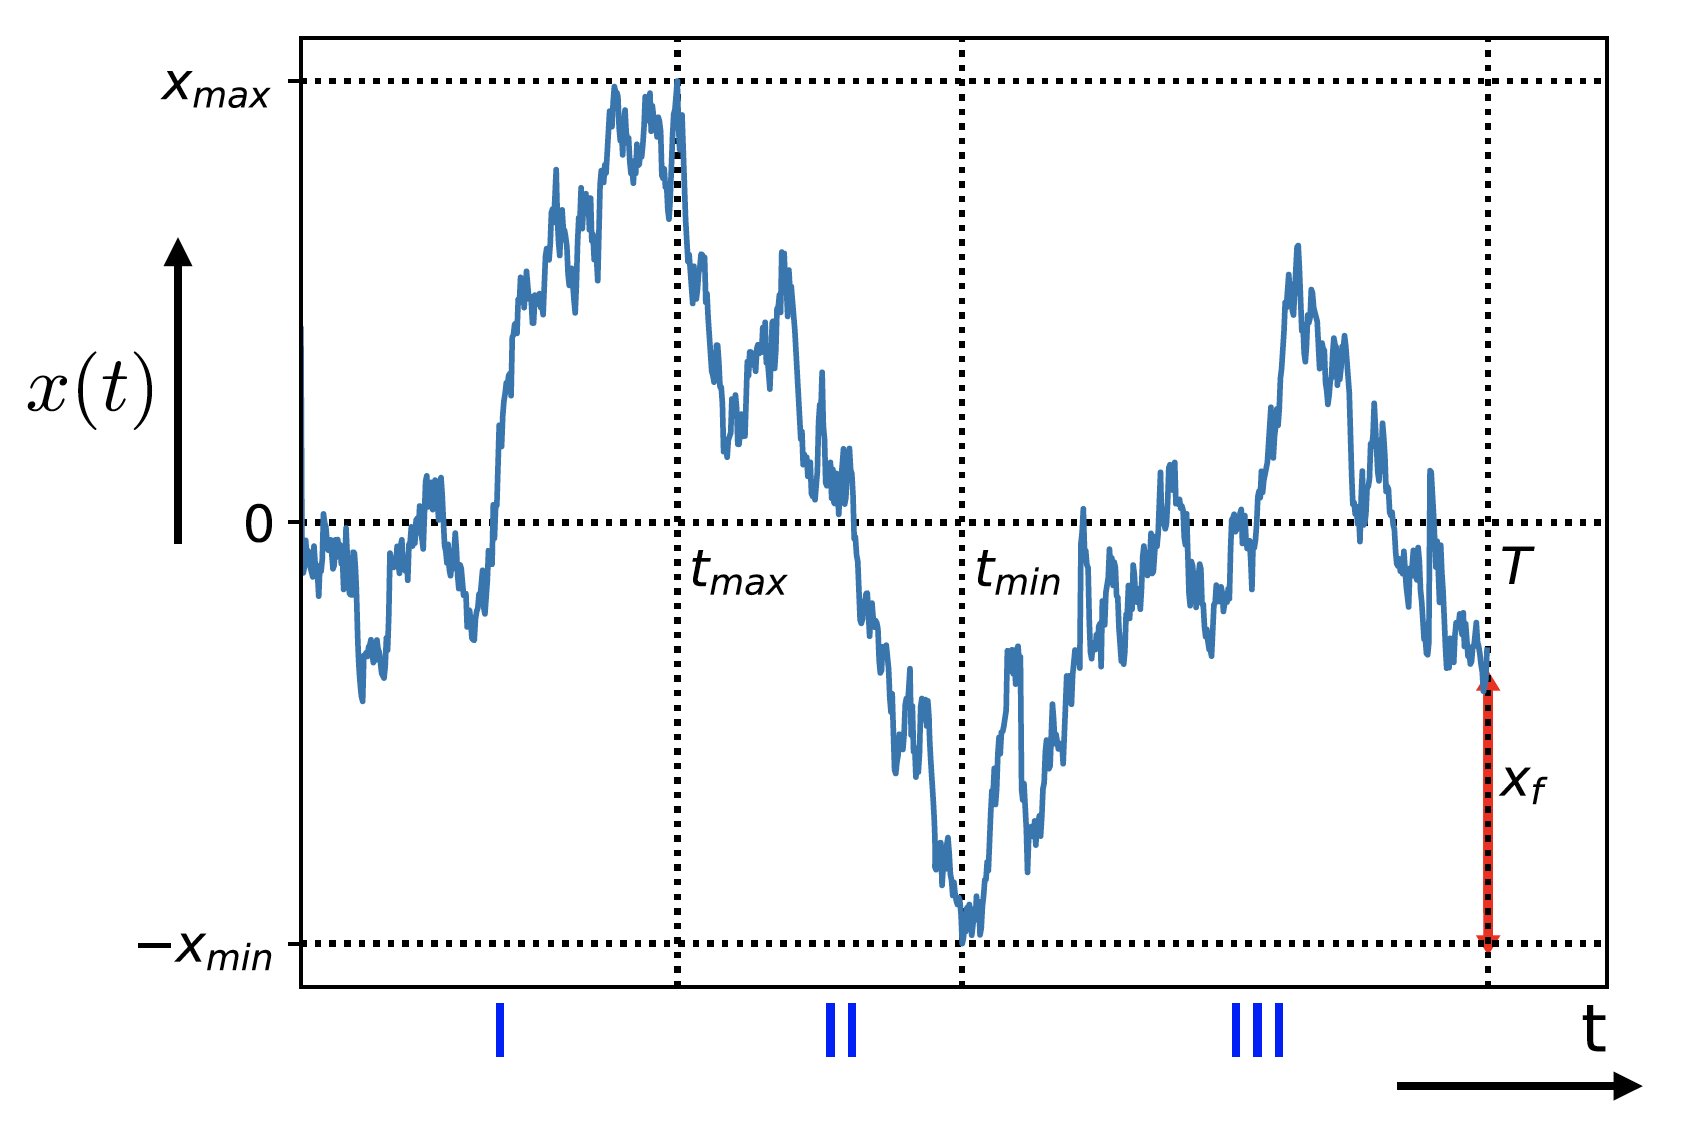
\includegraphics[width=0.65\linewidth]{BM.png}
  	\caption{Illustration of three r.v.s.}
  	\label{BM}
	\end{figure}
\end{frame}

\begin{frame}{L\'{e}vy's arcsine law}
\par
\begin{Thm}[L\'{e}vy’s arcsine law\footnotemark, 1940]\label{levy}
    Three r.v.s defined above obey the same law as follows:
    \begin{equation}
        p\lp x \rp = \frac{1}{\pi\sqrt{x\lp 1 - x \rpz}}, \quad x \in \lb 0, 1 \rb.
    \end{equation}
\end{Thm}
\footnotetext{P. L\'evy. Sur certains processus stochastiques homog\`enes. Compositio mathematica, 7:283–339, 1940.}
\end{frame}


\begin{frame}{L\'{e}vy's arcsine law}
\par
\begin{figure}[H]
	\centering
  	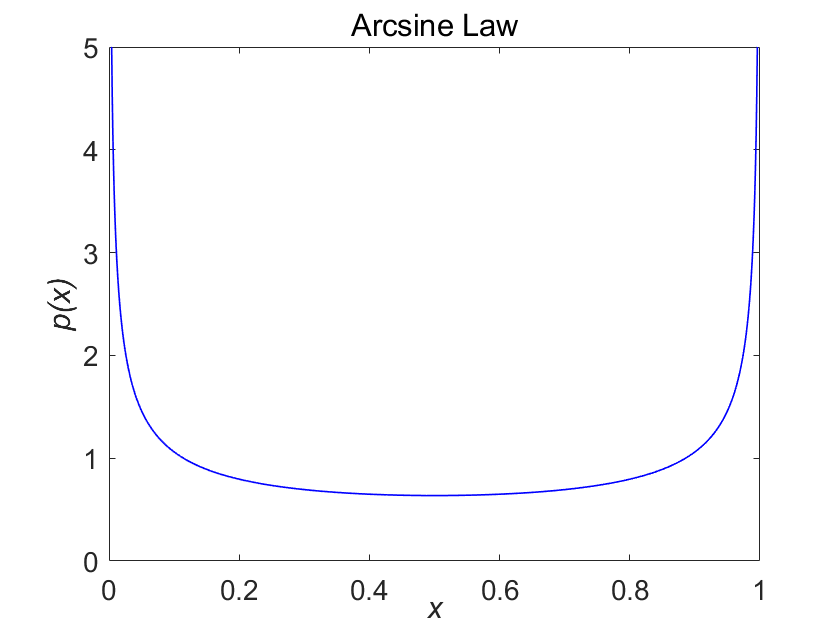
\includegraphics[width=10.6cm]{arcsine law.png}
\end{figure}
\end{frame}


\begin{frame}{Arcsine law for Markov chain: Combinatorial approach}
\par
Key insight: \textbf{Viewing Brownian motion as a sum of an i.i.d. sequence!}
\par
A comparison between Brownian motion on $\mbR$ and general Markov chain:
\begin{itemize}
    \item 1. Brownian motion on $\mbR$: order relation, $0$, positivity \& negativity, maximum \& minimum.     \\
    \item 2. Markov chain on $\Omega$: discrete state space without order relation.     \\
\end{itemize}
\par
Solution: Consider functional on Markov chain $f: \Omega \rightarrow \mbR$ and use induced order relation.
\end{frame}


\begin{frame}{Combinatorial approach}
\small
\begin{Thm}[Arcsine law for i.i.d.\ sequence\footnotemark, 1956]
Let $X_1, \cdots, X_n$ be i.i.d. r.v.s. Denote $S_k = \sum_{i = 1}^k X_i$ as their partial sum, $a_i = P\lp S_i > 0 \rp$, and $r_N = \frac{\#\lbb i \big| S_i > 0, 1 \leq i \leq N \rbb}{N}$. Suppose $\frac{\sum_{i = 1}^n a_i}{n} \rightarrow \alpha$, then
\begin{equation}
P(r_N \leq x) \rightarrow  F_{\alpha}\lp x \rp,
\end{equation}
where $F_{\alpha}\lp x \rp$ is the generalized arcsine law given by
\begin{equation}
    F_{\alpha}\lp x \rp = \lbb 
    \begin{aligned}
        & \frac{\sin \pi \alpha}{\pi} \int_{0}^x s^{\alpha - 1}\lp 1 - s \rp^{\alpha - 1} \, \mathrm{d} s, \; & 0 \leqslant x \leqslant 1, \\
        & 0, & x < 0,       \\
        & 1, & x > 1.
    \end{aligned}\right.
\end{equation}
\end{Thm}
\begin{Rem}
    Taking $\alpha = \half$, we obtain the ordinary arcsine law of L\'evy Thm\eqref{levy}.
\end{Rem}
\footnotetext{F.  Spitzer.  A  combinatorial  lemma  and  its  application  to  probability  theory. Transactions of the American Mathematical Society, 82(2):323–339, 1956.}


\end{frame}


\begin{frame}{ Combinatorial approach}
Consider an aperiodic, positive recurrent irreducible discrete Markov chain $\lbb X_n, \Omega, P \in \mbR^{\lv \Omega \rv \times \lv \Omega \rv}, \pi \in \mbR^{\lv \Omega \rv} \rbb$. $f: \Omega \rightarrow \mbR$ is a functional on this chain. 
\par
Suppose $X_0 = i \in \Omega$, denote the $n$-th time this chain comes back to state $i$ by $\tau_i$, so that $\tau_1 = 0$. And define $\eta_{\nu} = \tau_{\nu + 1} - \tau_{\nu}$. One has $\frac{1}{\pi_i} = \mbE\eta_{\nu}, \ \forall \nu$. Introduce a r.v. on each time interval as
\begin{equation}
    Y_{\nu} = \sum_{s = \tau_{\nu}}^{\tau_{\nu + 1} - 1} f\lp X_s \rp, \quad \nu = 1, 2, \cdots.
\end{equation}
\end{frame}


\begin{frame}{Combinatorial approach}
Then if $\sum_{i \in \Omega} \pi_i f\lp i \rp < \infty$, we know that $M = \pi_i \mbE Y_{\nu}$ is finite. Now let $\bar{f} = f - M$ and $Z_{\nu} = Y_{\nu} - \rho_{\nu}M$. As before, $Z_{\nu}, Y_{\nu}, \nu = 1,2,\cdots$ are a sequence of i.i.d. r.v.s. Write $\hat{S}_{\nu} = \sum_{s = 1}^{\nu} Z_s$. Finally put $\bar{S}_n = \sum_{s = 0}^n \bar{f}\lp X_s \rp$. And define the r.v. indicating the ratio of positive numbers in $\bar{S}_n$, i.e.
\begin{equation}
    r_N  = \frac{\# \lbb \nu = 0,1, \cdots, N \big| \bar{S}_{\nu} > 0 \rbb}{N}.
\end{equation}
Suppose the limit exists $\lim_{n \rightarrow \infty} \frac{1}{n} \sum_{\nu = 1}^n P\lp \bar{S}_{\nu} > 0 \rp = \alpha$.
\begin{Thm}[Arcsine law for Markov chain\footnotemark, 1963]
    With above definition, we have
    \begin{equation}
P(r_N \leq x) \rightarrow  F_{\alpha}\lp x \rp.
\end{equation}
\end{Thm}
\footnotetext{D. A. Freedman. An arcsine law for markov chains.Proceedings of the American Mathematical Society,14(4):680–684, 1963.}
\end{frame}


\begin{frame}{Arcsine law for Markov chain: Law for thermodynamics current}
\par
Recently, Barato et al. derive an arcsine law for thermodynamic currents, which has relation with thermodynamics uncertainty relation.
\par
Specifically, define integrated fluctuating current:
\begin{equation}
    J_N \simeq \sum_{i,j}d_{ij}\mathcal{N}_{ij}.
\end{equation}
with $\mathcal{N}_{ij}\simeq \sum_{n=1}^N \delta_{i,i_{n-1}}\delta_{j,i_n}$ where $i_n$ refers to the state where sample path arrive at time $n$, and $d_{ij}$s are supposed to be bounded constant, $\delta$ is Kronecker symbol. Define random variable $\mathcal{R}_N \simeq \frac{1}{N}\sum_{n=1}^N \theta(J_n-\mbE(J_n))$ with $\theta\lp x \rp = \mathbf{1}_{\lb 0, \infty \rp}$ the characteristic function.

\end{frame}


\begin{frame}{Law for thermodynamics current}
\begin{Thm}[Arcsine law for Markov chain\footnotemark, 2018]
    With above definition, we have
    \begin{equation}
P(\mathcal{R}_N \leq x) \rightarrow  \frac{1}{\pi\sqrt{x\lp 1 - x \rpz}}, \quad x \in \lb 0, 1 \rb.
\end{equation}
\end{Thm}
\begin{proof}[Proof idea]\renewcommand{\qedsymbol}{}
    To prove this result, we introduce an auxiliary Markov chain $Z_n$ in the following way: the state space of this chain is $\Omega_Z=\{z_{ij}P_{ij} \textgreater 0\}$, and the transition probabilities of this chain is $p_{z_{ij}z_{kl}}=\delta_{jk}P_{jl}$. Then by elementary Markov chain theory we have that $Z_n$ is also irreducible, aperiodic and positive recurrent with invariant distribution: $\pi_{z_{ij}}=\pi_i P_{ij}$.
\end{proof}
\footnotetext{A. C. Barato, \'E. Rold\'an, I. A. Mart\'inez, and S. Pigolotti. Arcsine laws in stochastic thermodynamics.Physical review letters, 121(9):090601, 2018.}
\end{frame}


\begin{frame}{Law for thermodynamics current}
\begin{proof}[(Continue)]
Thus it's trivial that $\mathcal{N}_{ij} = \sum_{n=1}^N \delta_{z_{ij},z_{i_{n-1}i_n}} = \sum_{n=1}^N \mathbf{1}_{ij}\lp Z_n \rp$. Therefore, denote a functional on auxiliary chain $Z_n$ as $f: \Omega_Z \rightarrow \mbR, f\lp z_{ij} \rp = d_{ij}$, the current $J_N$ can be rewritten as:
\begin{equation}\label{current-2}
J_N = \sum_{z_{ij} \in \Omega_Z}f(z_{ij})\mathcal{N}_{ij} = \sum_{n = 1}^N f\lp Z_n \rp.
\end{equation}
And the problem is translated to the one already proved by Freedman. The only ingredient $\lim_{n \rightarrow \infty}P\lp S_n > 0 \rp = \half$ to guarantee the classical arcsine law is a corolary of the central limit theorem for Markov chain\footnotemark.
\end{proof}
\footnotetext{G. L. Jones et al. On the markov chain central limit theorem. Probability surveys, 1:299–320, 2004.}
\end{frame}


\begin{frame}{Law for thermodynamics current}
\begin{Rem}[Possible connection with statistical thermodynamics]
    Entropy production rate, an essential quantity \footnotemark in statistical thermodynamics, falls in this framework. In its simplest form in Markov chain, it reads $\sigma = \sum_{i, j} \mcN_{ij} \log \frac{W_{ij}}{W_{ji}}$. This kind of arcsine law may bridge a connection to the thermodynamics uncertainty relation\footnotemark, which usually take the form
\begin{equation}\label{uncertain}
    \frac{\Var\lp J \rp}{\la J \ra^2} \geq \frac{2}{T\sigma},
\end{equation}
where $T$ is the length of time interval and $\sigma$ the entropy production rate.
\end{Rem}
\footnotetext{G. E. Crooks. Entropy production fluctuation theorem and the nonequilibrium work relation for free
energy differences. Phys. Rev. E, 60:2721–2726, Sep 1999.}
\footnotetext{T. R. Gingrich, J. M. Horowitz, N. Perunov, and J. L. England. Dissipation bounds all steady-state
current fluctuations. Physical review letters, 116(12):120601, 2016.}
\end{frame}


\begin{frame}{Arcsine law for Markov chain: Jump process}
\par
The generalization to jump process is direct. Consider an aperiodic, positive recurrent, regular Markov jump process $\lbb X_t, \Omega, \right.$ $\left.Q \in \mbR^{\lv \Omega \rv \times \lv \Omega \rv},  \pi \in \mbR^{\lv \Omega \rv} \rbb$. Specifically, one can define integrated fluctuating current:
\begin{equation}
    J_T \simeq \sum_{i,j}d_{ij}\mathcal{N}_{ij},
\end{equation}
up to a time bound $T$ and consider all the transition that happen before $T$. Define random variable $\mathcal{R}_T \simeq \frac{1}{T} \int_0^T \theta(X_t-E(X_t))dt$ with $\theta\lp x \rp = \mathbf{1}_{\lb 0, \infty \rp}$ the characteristic function. It is simple to show this integral is well-defined even in Riemannian sense.

\end{frame}


\begin{frame}{Arcsine law for Jump process}
\par

\begin{Thm}[Arcsine law for jump processes]
    With above definition, we have
    \begin{equation}
P(\mathcal{R}_N \leq x) \rightarrow  \frac{1}{\pi\sqrt{x\lp 1 - x \rpz}}, \quad x \in \lb 0, 1 \rb.
\end{equation}
\end{Thm}
\begin{proof}[Proof idea]\renewcommand{\qedsymbol}{}
    \begin{itemize}
    	\item 1. Construct auxiliary chain.
	\item 2. Use strong Markov property to translate to conclusion on i.i.d. sequence.
	\item 3. Use law of large number to deal with the details in time duration of each travel.
    \end{itemize}
\end{proof}

\end{frame}


\begin{frame}{Arcsine law for Markov chain: Lamperti's Topological approach}
\par
Viewing the classical arcsine law as law of occupation time, i.e. time spend in a given set.
\par
The topological property is the essence of distribution of occupation time. One can consider Markov chain with similar topological structure, i.e. $\Omega = A \sqcup B \sqcup \{ \sigma \}$. The chain can not transfer from $A(B)$ to $B(A)$ without passing $\{ \sigma \}$. Topologically speaking, $\Omega$ is path-connected while $\Omega \backslash \{ \sigma \}$ is not.
\end{frame}


\begin{frame}{Setting of Lamperti's Topological approach}
\par
Now, consider a Markov chain $\{X_n, X_n \in \Omega \}$ on this state space with $X_0 = \sigma$. We assume that the state $\sigma$ is a recurrent state, with $f_n$ denoting the probability of recurrence time of $\sigma$ is $n$. Denote the generating function as $F\lp x \rp = \sum_{i = 1}^{\infty} f_i x^i$. We denote the occupation time of $A$ up to time $n$ as $T_n^{A}$, with the convention that occupation of $\sigma$ is counted or not according to whether the last other state occupied is in $A$ or not. 
\end{frame}


\begin{frame}{Lamperti's Topological approach}
	\begin{Thm}[Lamperti’s generalized arcsine law\footnotemark, 1958]
Let $X_n$ be the process defined above. Then
    \begin{equation}
\lim_{n \rightarrow \infty}P\lp\frac{T_n^A}{n} \leq t \rp =  G_{\alpha, \delta}\lp t \rp,
    \end{equation}
    where $\lim_{n \rightarrow \infty}\mbE \frac{T_n^A}{n} = \delta, \lim_{x \rightarrow 1^-} \frac{\lp 1 - x \rp F'\lp x \rp}{1 - F\lp x \rp} = \alpha$ and the p.d.f.\ $G_{\alpha}'\lp x \rp$ is the generalized arcsine law given by
\begin{equation}
    G_{\alpha, \delta}'\lp x \rp = \frac{a\sin \pi \alpha}{\pi} \frac{x^{\alpha}\lp 1 - x \rp^{\alpha - 1} + x^{\alpha - 1}\lp 1 - x \rp^{\alpha}}{a^2x^{2\alpha} + 2ax^{\alpha}\lp 1 - x \rp^{\alpha}\cos \pi \alpha + \lp 1 - x \rp^{2\alpha}},
\end{equation}
where $a = \frac{1 - \delta}{\delta}$.
\end{Thm}
\footnotetext{J. Lamperti. An occupation time theorem for a class of stochastic processes. Transactions of the American Mathematical Society, 88(2): 380–387, 1958.}
\end{frame}


\begin{frame}{Lamperti's Topological approach}
	\begin{Rem}
		When both the parameters $\alpha, \delta$ are given by $\half$ (hence $a = 1$), the generalized arcsine law reduces to classical arcsine law as follows
		\bequn
			\begin{aligned}
				G_{\half, \half}'\lp x \rp = & \ \frac{1}{\pi} \frac{\sqrt{\frac{x}{1 - x}} + sqrt{\frac{1 - x}{x}}}{x + 1 - x}		\\
				= & \ \frac{1}{\pi} \lp \sqrt{\frac{x}{1 - x}} + sqrt{\frac{1 - x}{x}} \rp 		\\
				= & \ \frac{1}{\pi\sqrt{x\lp 1 - x \rp}}.
			\end{aligned}
		\eequn
	\end{Rem}
\end{frame}


\begin{frame}{Lamperti's Topological approach}
    	\begin{figure}[H]
	\centering
  	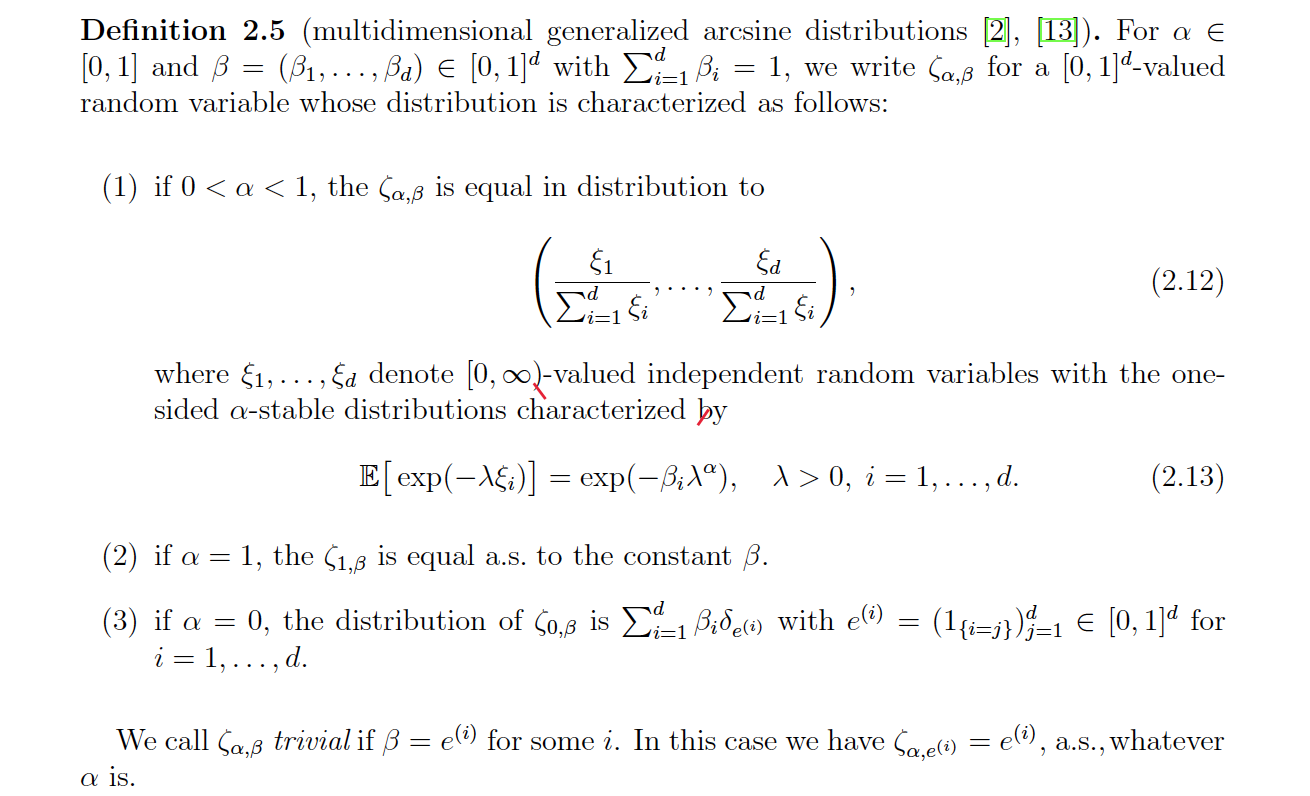
\includegraphics[width=\linewidth]{multi1.png}
  	\caption{Multidimensional generalized arcsine law}
  	\label{multi-def}
	\end{figure}
\end{frame}


\begin{frame}{Lamperti's Topological approach}
    	\begin{figure}[H]
	\centering
  	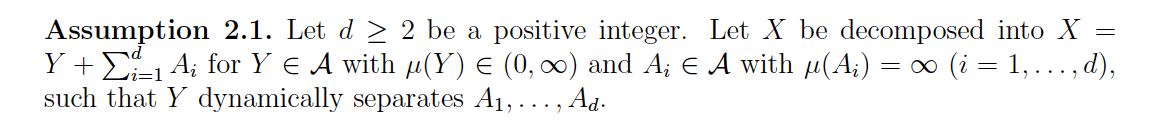
\includegraphics[width=\linewidth]{assum1.png}
  	%\caption{Assumption 1}
  	\label{multi-assum1}
	\end{figure}
	\begin{figure}[H]
	\centering
  	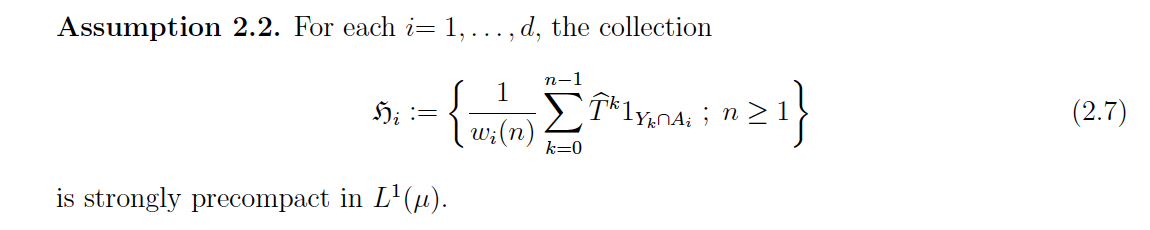
\includegraphics[width=\linewidth]{assum2.png}
  	%\caption{Assumption 2}
  	\label{multi-assum2}
	\end{figure}
	\begin{figure}[H]
	\centering
  	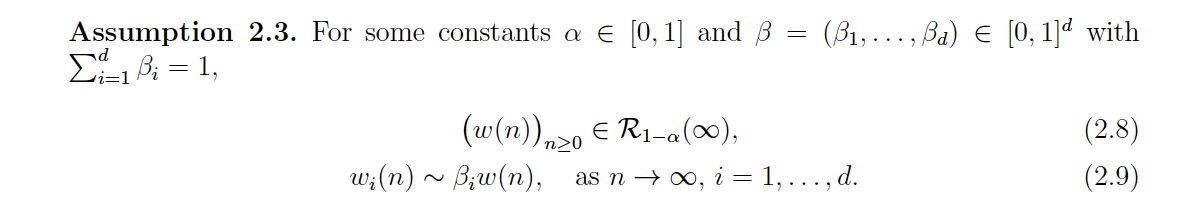
\includegraphics[width=\linewidth]{assum3.png}
  	\caption{Assumptions}
  	\label{multi-assum3}
	\end{figure}
\end{frame}


\begin{frame}{Lamperti's Topological approach}
    	\begin{figure}[H]
	\centering
  	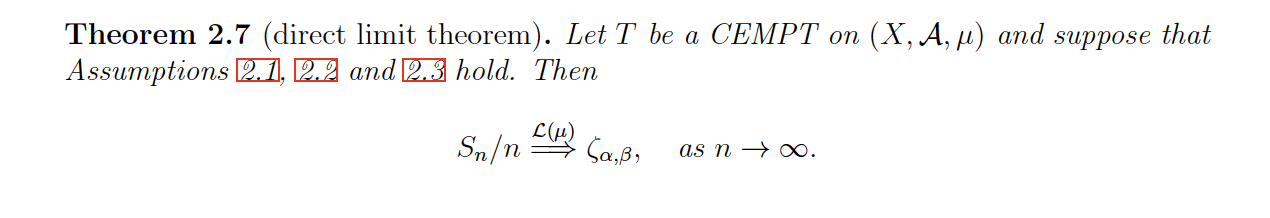
\includegraphics[width=\linewidth]{multi2.png}
  	\caption{Direct limit theorem}
  	\label{multi-direct}
	\end{figure}
	\begin{figure}[H]
	\centering
  	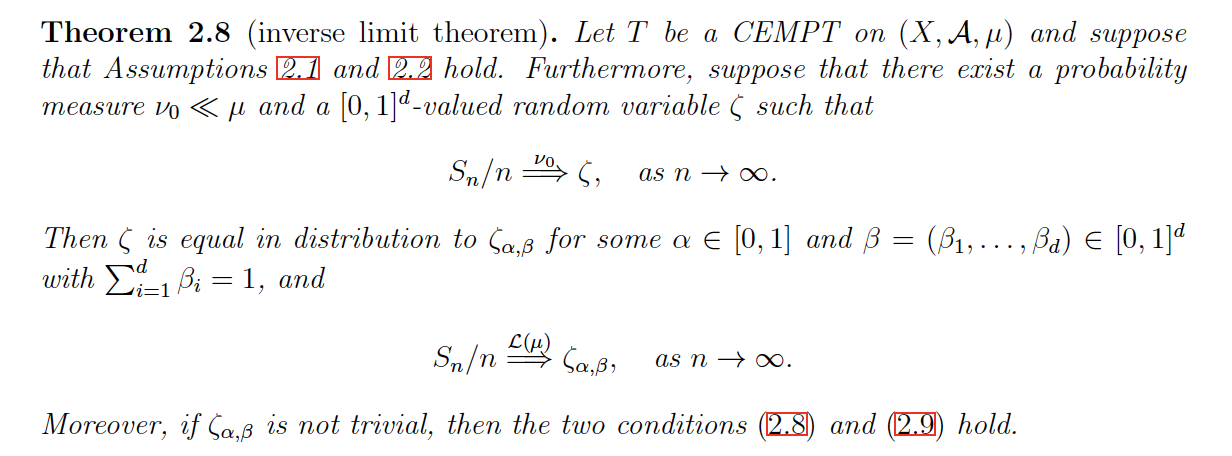
\includegraphics[width=\linewidth]{multi3.png}
  	\caption{Inverse limit theorem}
  	\label{multi-inv}
	\end{figure}
\end{frame}


\begin{frame}{Arcsine law in high time dimension: Extreme statistics in Gaussian free field}
	\par
	\bequn
		\begin{aligned}
			\text{Random walk on $\mbZ$} & \Longrightarrow  \text{Random walk on $\mbZ^d$},		\\
			\text{Random walk on $\mbZ$} & \Longrightarrow  \text{Gaussian free field on $\mbZ^d$}.
		\end{aligned}
	\eequn
	Firstly, we review some basic definition concerned with GFF. 
	\begin{figure}[H]
	\centering
  	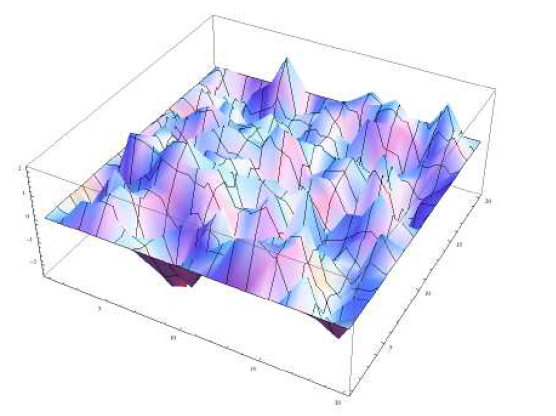
\includegraphics[width=0.45\linewidth]{GFF.png}
  	\caption{Gaussian Free Field}
  	\label{GFF}
	\end{figure}
\footnotetext{S. Sheffield. Gaussian free fields for mathematicians. Probability theory and related fields, 139(3-4):521–
541, 2007.}
\end{frame}


\begin{frame}{Extreme statistics in Gaussian free field}
	A discrete two-dimensional Gaussian free field (GFF) on a $2D$ box $V_N := \lp \lb 0, N - 1 \rb \cap \mbZ \rp^2$ of side length $N$ with Dirichlet boundary condition, is a mean zero Gaussian process indexed by $V_N$ which takes the value $0$ on $\p V_N$ satisfies either of the following:
	\begin{itemize}
		\item 1. density function given by
		\bequ
			f\lp \lp \eta_v \rp_{v \in V_N} \rp = Ze^{-\frac{\sum_{u \sim v}\lp \eta_u - \eta_v \rp^2}{16}}.
		\eequ
		\item 2. Its covariance matrix is given by $G_{\p V_N}\lp x, y \rp$, where $G_{\p V_N}\lp u, v \rp$ is the Green function defined by
		\bequn	
			\begin{aligned}
				G_{\p V_N}\lp u, v \rp & = \mbE_u\lb \sum_{k = 0}^{\tau_{\p V_N - 1}} \mathbf{1}_{S_k = v}\rb,	\quad \forall u \in V_N \backslash \p V_N, v \in V_N, 	\\
				G_{\p V_N}\lp u, v \rp & = 0, \quad \forall u \in {\p V_N}, v \in V_N.
			\end{aligned}
		\eequn
	\end{itemize}
	Equivalence is a simple observation that the discrete Green function is the inverse of discrete Laplacian, a while known result in discrete harmonic analysis.
\end{frame}


\begin{frame}{Extreme statistics in Gaussian free field}
	We consider the maximum of the discrete two-dimensional GFF on $V_N$, and denote $M_N = \max_{v \in V_N} \eta_v^N, m_N = \mbE M_N.$
	\begin{Thm}[Expectation of Maximum\footnotemark, 2001]
		\begin{itemize}
			\item 1. $\lim_{N \rightarrow \infty}P\lp M_N \geq 2\sqrt{\frac{2}{\pi}}\log N\rp = 0$. 
			\item 2. $\forall \epsilon > 0, \forall \delta \in \lb 0, \half \rp, \exists c = c\lp \delta, \epsilon \rp > 0, s.t.$
			\bequ
				P\lp M_N \leq \lp 2\sqrt{\frac{2}{\pi}} - \epsilon \rp\log N \rp \leq -exp\lp -c\lp \log N \rp^2 \rp,
		\eequ
		where $V_N^{\delta} := \{ v \in V_N: \dist\lp v, \rp V_N \geq \delta N \}$ for $N$ large enough.
		\end{itemize}
	\end{Thm}
\footnotetext{E. Bolthausen, J.-D. Deuschel, G. Giacomin, et al. Entropic repulsion and the maximum of the two-
dimensional harmonic. The Annals of Probability, 29(4):1670–1692, 2001.}
\end{frame}


\begin{frame}{Extreme statistics in Gaussian free field}
	\begin{Thm}[Expectation of Maximum for GFF\footnotemark, 2012]
		\bequ
			m_N = 2\sqrt{\frac{2}{\pi}}\log_2 N - \frac{3}{4}\sqrt{\frac{2}{\pi}}\log_2 \log_2 N + O\lp 1 \rp.
		\eequ
	\end{Thm}
	\begin{Thm}[Expectation of Maximum for BRW\footnotemark, 1978]
		\bequ
			m_N = 2\sqrt{\log 2}\log_2 N - \frac{3\sqrt{\log 2}}{4}\log_2 \log_2 N + O\lp 1 \rp.
		\eequ
	\end{Thm}
\footnotetext{M. Bramson and O. Zeitouni. Tightness of the recentered maximum of the two-dimensional discrete
gaussian free field. Communications on Pure and Applied Mathematics, 65(1):1–20, 2012.}
\footnotetext{M. D. Bramson. Maximal displacement of branching brownian motion. Communications on Pure and Applied Mathematics, 31(5):531–581, 1978.}
\end{frame}


\begin{frame}{Extreme statistics in Gaussian free field}
	\begin{Thm}[Geometry of the set of near maxima\footnotemark, 2014]
		There exists an absolute constant $c > 0$, 
		\bequ
			\begin{aligned}
				\lim_{r \rightarrow \infty}\lim_{N \rightarrow \infty} P\lp  \exists v, u \in V_N: r \leq \lv v - u \rv \leq \frac{N}{r} \  \right. \\ \left. \eta_u^N, \eta_v^N \geq m_N - c\log\log r  \rp = 0.
			\end{aligned}
		\eequ
		\end{Thm}
		\begin{Thm}[Geometry of the set of near maxima\footnotemark, 2014]
		For $\lambda > 0$, let $A_{N, \lambda} = \{ v \in V_N: \eta_v \geq m_N - \lambda \}$ for $\lambda > 0$. Then there exist absolute constant $c, C$ s.t.
		\bequ
			\begin{aligned}
				\lim_{\lambda \rightarrow \infty}\lim_{N \rightarrow \infty} P\lp ce^{c\lambda} \leq \lv A_{N, \lambda} \rv \leq Ce^{C\lambda}  \rp = 1.
			\end{aligned}
		\eequ
		\end{Thm}
\footnotetext{J. Ding, O. Zeitouni, et al. Extreme values for two-dimensional discrete gaussian free field. The Annals of Probability, 42(4):1480–1515, 2014.}
\end{frame}


\begin{frame}{Extreme statistics in Gaussian free field}
	\begin{proof}[Proof idea]
		Completely different techniques comparing to Brownian motion case. 
		\par
		One key ingredient is to compare the extreme statistics of GFF with those of branching random walk (BRW) or modified branching random walk\footnotemark (MBRW). They share lots of similarity since they have the proportional covariance.
		\par
		Comparison of Gaussian processes.
	\end{proof}
\end{frame}

\begin{frame}{Extreme statistics in Gaussian free field}
\begin{Prop}[Similarity of covariance between GFF and BRW\footnotemark, 2012]
		There exists a constant $C$ s.t. $\forall x, y \in V_N$
		\bequ
			\begin{aligned}
				\lv \Cov_{GFF}^N\lp x, y \rp - \frac{2\log 2}{\pi}\lp n - \log_2 d^N\lp x, y \rp \rp \rv \leq C		,		\\
				\lv \Cov_{MBRW}^N\lp x, y \rp - \lp n - \log_2 d^N\lp x, y \rp \rp \rv \leq C,
			\end{aligned}
		\eequ
		where the distance is given by $d^N\lp x, y \rp = 
		\min_{z \sim y}\norml x - z \normr$.
	\end{Prop}
\footnotetext{M. Bramson and O. Zeitouni. Tightness of the recentered maximum of the two-dimensional discrete
gaussian free field. Communications on Pure and Applied Mathematics, 65(1):1–20, 2012.}
\end{frame}


\begin{comment}
\begin{frame}{Generalized arcsine law: double Laplace transform formula}
	\begin{equation}\label{double-laoplace}
	\begin{aligned}
    & \ \int_0^{\infty} e^{-\mu t} \mbE\lb \exp\lbb -\sum_{i = 1}^N \lambda_i A_i\lp t \rp \rbb \rb dt \\
    = & \ \frac{1}{\sum_{i = 1}^N \psi\lp \lambda_i + \mu \rp}\lp \sum_{i = 1}^N \frac{\psi\lp \lambda_i + \mu \rp}{\lambda_i + \mu} \rpz.
    \end{aligned}
\end{equation}
\end{frame}
\end{comment}


\begin{frame}
	Thanks for listening.
\end{frame}


\begin{comment}
\begin{frame}{Generalized arcsine law: $t_{\max}$ of stochastic processes}
The distribution of $t_{\max}$ of the following stochastic processes is calculated by the methods of path-integral\footnote{S. N. Majumdar and J.-P. Bouchaud. Optimal time to sell a stock in the Black-Scholes model: comment on 'Thou shalt buy and hold', by Shiryaev, Z. Xu and X. Y. Zhou. Quant.\ Finance 8, 753 (2008).}\textsuperscript{,}\footnote{S. N. Majumdar, J. Randon-Furling, M. J. Kearney and M. Yor. On the time to reach maximum for a variety of constrained Brownian motions. J. Phys.\ A 41, 365005 (2008).}, agreement formulae\textsuperscript{7} and renormalization group\footnote{G. Schehr and P. Le Doussal. Extreme value statistics from the real space renormalization group: Brownian motion, Bessel processes and continuous time random walks. J. Stat.\ Mech.\ (2010) P01009.}.
\begin{itemize}
	\item 1. Brownian bridge, reflected Brownian bridge, Brownian excursion, Brownian meander, Brownian motion with drift, Bessel process, Bessel bridge.
	\item 2. Discrete-time random walk.
	\item 3. Run-and-tumble particle.
\end{itemize}
\end{frame}


\begin{frame}{Generalized arcsine law: $t_{\max}$ of Brownian bridge and reflected Brownian bridge}
Denote $X_t^\text{bri}$ as a Brownian bridge on $[0,T]$, which is defined as a Brownian motion, $X_t$, constrained such that $X_0 = 0$ and $X_T = 0$. Define $X_t^\text{ref bri} := \left|X_t^\text{bri}\right|$ which denotes a reflected Brownian bridge on $[0,T]$. The time of the maximum is denoted by:
\begin{equation}
    \begin{aligned}
        t_\text{max}^\text{bri} & := \frac{1}{T}\arg \max_{t \in [0, T]} X_t^\text{bri},  \\
        t_\text{max}^\text{ref bri} & := \frac{1}{T}\arg \max_{t \in [0, T]} X_t^\text{ref bri}.
    \end{aligned}
\end{equation}
\end{frame}

\begin{frame}{Generalized arcsine law: $t_{\max}$ of Brownian bridge and reflected Brownian bridge}
\begin{Thm}[Distribution of $t_{\max}$ of Brownian bridge\footnotemark, 1957]
$t_\text{max}^\text{bri}$ obeys uniform distribution
:
\begin{equation}
    p(x) = 1, \quad x \in [0, 1].
\end{equation}
\end{Thm}
\footnotetext{W. Feller. An introduction to probability theory and its applications. John Wiley and Sons, Inc.\ 1957.}
\end{frame}

\begin{frame}{Generalized arcsine law: $t_{\max}$ of Brownian bridge and reflected Brownian bridge}
\begin{Thm}[Distribution of $t_{\max}$ of reflected Brownian bridge\footnotemark, 2008]
$t_\text{max}^\text{ref bri}$ obeys the law as follows:
\begin{multline}
    p(x) = 2\sum_{n,m=0}^\infty (-1)^{m+n} \frac{(2m+1)(2n+1)}{\left[(2n+1)^2x+(2m+1)^2(1-x)\right]^{3/2}}, \\
    x \in [0, 1].
\end{multline}
\end{Thm}
\footnotetext{S. N. Majumdar, J. Randon-Furling, M. J. Kearney and M. Yor. On the time to reach maximum for a variety of constrained Brownian motions. J. Phys.\ A 41, 365005 (2008).}
\end{frame}

\begin{frame}{Generalized arcsine law: $t_{\max}$ of Brownian excursion and Brownian meander}
Denote $X_t^\text{ex}$ as a Brownian excursion on $[0,T]$, which is defined as a Brownian motion, $X_t$, constrained so that $X_0 = 0, X_T = 0$ with $X_t > 0$ for $t \in (0,T)$. Denote $X_t^\text{mea}$ as a Brownian meander on $[0,T]$, which is defined as a Brownian motion, $X_t$, constrained so that $X_0 = 0$ with $X_t > 0$ for $t \in (0,T]$. The time of the maximum is denoted by:
\begin{equation}
    \begin{aligned}
        t_\text{max}^\text{ex} & := \frac{1}{T}\arg \max_{t \in [0, T]} X_t^\text{ex},  \\
        t_\text{max}^\text{mea} & := \frac{1}{T}\arg \max_{t \in [0, T]} X_t^\text{mea}.
    \end{aligned}
\end{equation}
\end{frame}

\begin{frame}{Generalized arcsine law: $t_{\max}$ of Brownian excursion and Brownian meander}
\begin{Thm}[Distribution of $t_{\max}$ of Brownian excursion\footnotemark, 2008]
$t_\text{max}^\text{ex}$ obeys the law as follows:
\begin{equation}
    p(x) = 3\sum_{n,m=1}^\infty (-1)^{m+n} \frac{m^2n^2}{\left[n^2x+m^2(1-x)\right]^{5/2}}, \quad x \in [0, 1].
\end{equation}
\end{Thm}
\footnotetext{S. N. Majumdar, J. Randon-Furling, M. J. Kearney and M. Yor. On the time to reach maximum for a variety of constrained Brownian motions. J. Phys.\ A 41, 365005 (2008).}
\end{frame}

\begin{frame}{Generalized arcsine law: $t_{\max}$ of Brownian excursion and Brownian meander}
\begin{Thm}[Distribution of $t_{\max}$ of Brownian meander\footnotemark, 2008]
$t_\text{max}^\text{mea}$ obeys the law as follows:
\begin{equation}
    p(x) = 2\sum_{m=0,n=1}^\infty (-1)^{n+1} \frac{n^2}{\left[n^2x+(2m+1)^2(1-x)\right]^{3/2}}, x \in [0, 1].
\end{equation}
\end{Thm}
\footnotetext{S. N. Majumdar, J. Randon-Furling, M. J. Kearney and M. Yor. On the time to reach maximum for a variety of constrained Brownian motions. J. Phys.\ A 41, 365005 (2008).}
\end{frame}

\begin{frame}{Generalized arcsine law: $t_{\max}$ of Brownian motion with drift}
Define $X_t^{(\mu)} := X_t+\mu t$ which denotes a Brownian motion with drift on $\mbR$. The time of the maximum within the period $[0,T]$ is denoted by:
\begin{equation}
    t_\text{max}^{(\mu)} := \frac{1}{T}\arg \max_{t \in [0, T]} X_t^{(\mu)}.
\end{equation}
\end{frame}

\begin{frame}{Generalized arcsine law: $t_{\max}$ of Brownian motion with drift}
\begin{Thm}[Distribution of $t_{\max}$ of Brownian motion with drift\footnotemark, 2003]
$t_\text{max}^{(\mu)}$ obeys the law as follows:
\begin{multline}
    p(x;\Tilde{\mu}) = 2 \left[\frac{\varphi \left(\Tilde{\mu}\sqrt{x}\right)}{\sqrt{x}} + \Tilde{\mu}\Phi\left(\Tilde{\mu}\sqrt{x}\right)\right] \times \\
    \left[\frac{\varphi \left(\Tilde{\mu}\sqrt{1-x}\right)}{\sqrt{1-x}} - \Tilde{\mu}\Phi\left(-\Tilde{\mu}\sqrt{1-x}\right)\right], x \in [0, 1],
\end{multline}
where $\Tilde{\mu} = \mu \sqrt{T}$ and $\varphi (y) = \frac{1}{\sqrt{2\pi}}e^{-y^2/2}$, $\Phi (z) = \int_{-\infty}^z \varphi (y) \, \mathrm{d} y$ denote the standard Gaussian density and distribution function respectively.
\end{Thm}
\footnotetext{E. Buffet. On the time of the maximum of Brownian motion with drift. J. Appl.\ Math.\ Stoch.\ Anal.\ 16, 201 (2003).}
\end{frame}

\begin{frame}{Generalized arcsine law: $t_{\max}$ of Bessel process and Bessel bridge}
Denote $X_t^\text{Bes}$ as a Bessel process on $\mbR$, i.e.\ the radius of the $d$-dimensional Brownian motion $X_t^\text{Bes} = \sqrt{\sum_{i=1}^d (X_t^i)^2} + X_0^\text{Bes}$, where $X_t^1,X_t^2,\dots ,X_t^d$ are $d$ independent Brownian motion, $X_0^\text{Bes} \geqslant 0$. Denote $X_t^\text{Bes bri}$ as a Bessel bridge on $[0,T]$, which is defined as a Bessel process, $X_t^\text{Bes}$, constrained such that $X_0^\text{Bes} = 0$ and $X_T^\text{Bes} = 0$. Define the random variables as follows:
\begin{equation}
\begin{aligned}
    X_\text{max}^\text{Bes} & := \max_{t \in [0, T]} X_t^\text{Bes}, \\
    t_\text{max}^\text{Bes} & := \frac{1}{T}\arg \max_{t \in [0, T]} X_t^\text{Bes}, \\
    t_\text{max}^\text{Bes bri} & := \frac{1}{T}\arg \max_{t \in [0, T]} X_t^\text{Bes bri}.
\end{aligned}
\end{equation}
\end{frame}

\begin{frame}{Generalized arcsine law: $t_{\max}$ of Bessel process and Bessel bridge}
\begin{Thm}[Distribution of $t_{\max}$ of Bessel process\footnotemark, 2010]
$\left(t_\text{max}^\text{Bes}, X_\text{max}^\text{Bes}, X_T^\text{Bes}\right)$ obeys the law as follows:
\begin{multline}
    p(x,u,u_T;u_0,\nu) = \frac{4}{u^5} \frac{u_T^{\nu+1}}{u_0^\nu} \sum_{n,m=1}^\infty j_{\nu,n}j_{\nu,m} \frac{J_\nu (j_{\nu,n}\frac{u_0}{u}) J_\nu (j_{\nu,m}\frac{u_T}{u})}{J_{\nu+1}(j_{\nu,n}) J_{\nu+1}(j_{\nu,m})} \\
    e^{-\left[j_{\nu,n}^2x + j_{\nu,m}^2(1-x)\right]/u^2}, x \in [0,1],
\end{multline}
where $u = X_\text{max}^\text{Bes}/\sqrt{T}$, $u_T = X_T^\text{Bes}/\sqrt{T}$, $u_0 = X_0^\text{Bes}/\sqrt{T}$,
$\nu = -1+d/2$, $J_\nu (y)$ is the Bessel function of the first kind, and $0 < j_{\nu,1} < j_{\nu,2} < \cdots $ is the sequence of positive zeros of $J_\nu (y)$.
\end{Thm}
\footnotetext{G. Schehr and P. Le Doussal. Extreme value statistics from the real space renormalization group: Brownian motion, Bessel processes and continuous time random walks. J. Stat.\ Mech.\ (2010) P01009.}
\end{frame}

\begin{frame}{Generalized arcsine law: $t_{\max}$ of Bessel process and Bessel bridge}
\begin{Thm}[Distribution of $t_{\max}$ of Bessel bridge\footnotemark, 2010]
$t_\text{max}^\text{Bes bri}$ obeys the law as follows:
\begin{multline}
    p(x;\nu) = \sum_{n,m=1}^\infty \frac{4(1+\nu) j_{\nu,n}^{\nu+1} j_{\nu,m}^{\nu+1}}{J_{\nu+1}(j_{\nu,n}) J_{\nu+1}(j_{\nu,m}) \left[j_{\nu,n}^2x + j_{\nu,m}^2(1-x)\right]^{\nu+2}}, \\
    x \in [0, 1],
\end{multline}
where $\nu = -1+d/2$, $J_\nu (y)$ is the Bessel function of the first kind, and $0 < j_{\nu,1} < j_{\nu,2} < \cdots $ is the sequence of positive zeros of $J_\nu (y)$.
\end{Thm}
\footnotetext{G. Schehr and P. Le Doussal. Extreme value statistics from the real space renormalization group: Brownian motion, Bessel processes and continuous time random walks. J. Stat.\ Mech.\ (2010) P01009.}
\end{frame}

\begin{frame}{Generalized arcsine law: $t_{\max}$, $t_{\min}$ and $t_{>0}$ of discrete-time random walk}
Denote $\{S_n\}$ as a discrete-time random walk, i.e.\ $S_0 = 0$, $S_n = X_1+X_2+\dots+X_n$ denote the sums of a sequence of i.i.d.\ random variables. For $n = 1,2,\dots$, define three random variables as follows:
\begin{equation}
\begin{aligned}
    L_n & := \min \left\{k = 0,1,\dots,n \middle\vert S_k = \max_{0 \leqslant i \leqslant n} S_i \right\}, \\
    M_n & := \max \left\{k = 0,1,\dots,n \middle\vert S_k = \min_{0 \leqslant i \leqslant n} S_i \right\}, \\
    N_n & := \# \left\{ k = 1,\cdots,n \middle\vert S_k > 0 \right\}.
\end{aligned}
\end{equation}
\end{frame}

\begin{frame}{Generalized arcsine law: $t_{\max}$, $t_{\min}$ and $t_{>0}$ of discrete-time random walk}
\begin{Thm}[Distribution of $t_{\max}$, $t_{\min}$ and $t_{>0}$ of discrete-time random walk\footnotemark, 1954]
For $n = 1,2,\dots$, $L_n$, $n-M_n$ and $N_n$ obey the same law as follows:
\begin{equation}
\begin{aligned}
    & P(K_n=n) = \sideset{}{^*} \sum_{k_1,\dots,k_n} \prod_{i=1}^n \frac{a_i^{k_i}}{k_i!i^{k_i}}, \;
    P(K_n=0) = \sideset{}{^*} \sum_{k_1,\dots,k_n} \prod_{i=1}^n \frac{(1-a_i)^{k_i}}{k_i!i^{k_i}}, \\
    & P(K_n=m) = P(K_m=m)P(K_{n-m}=0), \; 1 \leqslant m \leqslant n-1,
\end{aligned}
\end{equation}
where $K_n = L_n$, $n-M_n$, or $N_n$, $a_n = P(S_n > 0)$, and the symbol $\sum_{k_1,\dots,k_n}^*$ indicates that the summation is restricted to those values of the summation variables $k_1,\dots,k_n$ which satisfy the relation $k_1+2k_2+\dots+nk_n = n$, $k_i \geqslant 0$, $i=1,2,\dots,n$.
\end{Thm}
\footnotetext{E. S. Andersen. On the fluctuations of sums of random variables II\@. Math.\ Scand, 2: 195, 1954.}
\end{frame}

\begin{frame}{Generalized arcsine law: $t_{\max}$, $t_{>0}$ and $t_{l-0}$ of run-and-tumble particle}
Denote $X_t^\text{RTP}$ as a run-and-tumble particle in one dimension, which is defined as follows:
\begin{multline}
X_0^\text{RTP} = 0, \; X_t^\text{RTP} = X_{T_{n-1}}^\text{RTP} + v_{n}(t-T_{n-1}), \;  T_{n-1} < t \leqslant T_n, \\
n = 1,2,\dots,
\end{multline}
where $v_1,v_2,\dots$ are i.i.d.\ random variables with each drawn from a symmetric PDF $W(v)$, and $T_n = \tau_1+\tau_2+\dots+\tau_n$ denote the sums of a sequence of i.i.d.\ random variables with each drawn from an exponential PDF $p(\tau) = \gamma e^{-\gamma\tau}, \tau \geqslant 0$ with parameter $\gamma$. 
\end{frame}

\begin{frame}{Generalized arcsine law: $t_{\max}$, $t_{>0}$ and $t_{l-0}$ of run-and-tumble particle}
Define three random variables as follows:
\begin{equation}
\begin{aligned}
    t_{>0}^\text{RTP} & := \frac{1}{T}\int_0^T \mathbf{1}_{\lb 0, \infty \rpz}\lp X_t^\text{RTP} \rp \, \mathrm{d} t,    \\
    t_{\max}^\text{RTP} & := \frac{1}{T}\arg \max_{t \in \lb 0, T \rb} X_t^\text{RTP},    \\
    t_{l-0}^\text{RTP} & := \frac{1}{T}\max_{t \in \lb 0, T \rb} \left\{ t \middle\vert X_t^\text{RTP} = 0 \right\}.
\end{aligned}
\end{equation}
\end{frame}

\begin{frame}{Generalized arcsine law: $t_{\max}$, $t_{>0}$ and $t_{l-0}$ of run-and-tumble particle}
\begin{Thm}[Distribution of $t_{\max}$ of run-and-tumble particle\footnotemark, 2020]
For symmetric $W(v)$, $t_{\max}^\text{RTP}$ obeys the law as follows:
\begin{multline} \label{eq:max of RTP}
    p(x;\gamma,T) = \gamma T S(xT) S\left((1-x)T\right) + S(T)\left(\delta(x)+\delta(1-x)\right), \\
    x \in [0,1],
\end{multline}
where
\begin{equation}
    S(y) = \frac{1}{2} e^{-\frac{\gamma y}{2}} \left(J_0\left(\frac{\gamma}{2}y\right) + J_1\left(\frac{\gamma}{2}y\right)\right),
\end{equation}
$J_0(y)$ and $J_1(y)$ are modified Bessel functions of the first kind.
\end{Thm}
\footnotetext{F. Mori, P. Le Doussal, S. N. Majumdar and G. Schehr. Universal properties of a run-and-tumble particle in arbitrary dimension. Cond.\ Mat.\ Stat.\ Mech. ArXiv:2006.06989v1, 2020.}
\end{frame}

\begin{frame}{Generalized arcsine law: $t_{\max}$, $t_{>0}$ and $t_{l-0}$ of run-and-tumble particle}
\begin{Thm}[Distribution of $t_{>0}$ and $t_{l-0}$ of run-and-tumble particle\footnotemark, 2019]
For the simple case with $W(v) = \left(\delta(v+v_0) + \delta(v-v_0)\right)/2$, $t_{>0}^\text{RTP}$ obeys the same law \eqref{eq:max of RTP} with $t_{\max}^\text{RTP}$, and $t_{l-0}^\text{RTP}$ obeys the law as follows:
\begin{equation}
    p(x;\gamma,T) = \gamma T S(xT) S\left((1-x)T\right) + 2S(T)\delta(x), \quad x \in [0,1],
\end{equation}
where
\begin{equation}
    S(y) = \frac{1}{2} e^{-\frac{\gamma y}{2}} \left(J_0\left(\frac{\gamma}{2}y\right) + J_1\left(\frac{\gamma}{2}y\right)\right),
\end{equation}
$J_0(y)$ and $J_1(y)$ are modified Bessel functions of the first kind.
\end{Thm}
\footnotetext{P. Singh and A. Kundu. Generalised 'arcsine' laws for run-and-tumble particle in one dimension. J. Stat.\ Mech.\ 2019(8): 083205, 2019.}
\end{frame}


\begin{frame}{Generalized arcsine law: $t_{\max}$ and $t_{\min}$ of stochastic processes}
The joint distribution of $t_{\max}$ and $t_{\min}$ of Brownian motion and Brownian bridge is calculated by the path-integral technique\footnote{F. Mori, S. N. Majumdar and G. Schehr. Time between the maximum and the minimum of a stochastic process. Phys.\ Rev.\ Lett.\ 123, 200201 (2019).} and reflection principle. In the case of discrete-time random walk, we prove the convergence of $t_\text{max}$ and $t_\text{min}$ in distribution while the conditions of Donsker's theorem are satisfied.
\end{frame}

\begin{frame}{Generalized arcsine law: $t_{\max}$ and $t_{\min}$ of Brownian motion and Brownian bridge}
Analogous to the definition of $t_{\max}$ and $t_\text{max}^\text{bri}$, the time of the minimum is denoted by:
\begin{equation}
\begin{aligned}
    t_\text{min} & := \frac{1}{T}\arg \min_{t \in [0, T]} X_t,  \\
    t_\text{min}^\text{bri} & := \frac{1}{T}\arg \min_{t \in [0, T]} X_t^\text{bri},
\end{aligned}
\end{equation}
where $X_t$ and $X_t^\text{bri}$ denote the standard Brownian motion and Brownian bridge on $[0,T]$ respectively.
\end{frame}

\begin{frame}{Generalized arcsine law: $t_{\max}$ and $t_{\min}$ of Brownian motion and Brownian bridge}
\begin{Thm}[Joint distribution of $t_{\max}$ and $t_{\min}$ of Brownian motion\footnotemark, 2019]
$(t_\text{max},t_\text{min})$ obeys the law as follows:
\begin{multline}\label{thm:max and min of BM}
    p(x_1,x_2) = \frac{4}{\pi^2} \sum_{n_1,n_2,n_3=1}^\infty \frac{(-1)^{n_2+1} n_2^2 \left[1-(-1)^{n_1}\right] \left[1-(-1)^{n_3}\right]} {\left[n_1^2x_1+n_2^2(x_2-x_1)+n_3^2(1-x_2)\right]^2}, \\
    x_1 \leqslant x_2, x_1,x_2 \in [0,1],
\end{multline}
where $x_1 = \min \{t_\text{max},t_\text{min}\}$ and $x_2 = \max \{t_\text{max},t_\text{min}\}$.
\end{Thm}
\footnotetext{F. Mori, S. N. Majumdar and G. Schehr. Time between the maximum and the minimum of a stochastic process. Phys.\ Rev.\ Lett.\ 123, 200201 (2019).}
\end{frame}

\begin{frame}{Generalized arcsine law: $t_{\max}$ and $t_{\min}$ of Brownian motion and Brownian bridge}
\begin{Thm}[Joint distribution of $t_{\max}$ and $t_{\min}$ of Brownian bridge\footnotemark, 2019]
$(t_\text{max}^\text{bri},t_\text{min}^\text{bri})$ obeys the law as follows:
\begin{multline}
    p(x_1,x_2) = 3 \sum_{n_1,n_2=1}^\infty \frac{(-1)^{n_1+n_2}n_1^2n_2^2} {\left[n_1^2|x_1-x_2|+n_2^2\left(1-|x_1-x_2|\right)\right]^{5/2}}, \\
    x_1,x_2 \in [0,1].
\end{multline}
\end{Thm}
\footnotetext{F. Mori, S. N. Majumdar and G. Schehr. Time between the maximum and the minimum of a stochastic process. Phys.\ Rev.\ Lett.\ 123, 200201 (2019).}
\end{frame}

\begin{frame}{Generalized arcsine law: $t_{\max}$ and $t_{\min}$ of discrete-time random walk}
Denote $\{S_n\}$ as a discrete-time random walk, i.e.\ $S_0 = 0$, $S_n = X_1+X_2+\dots+X_n$, $X_1,X_2,\dots$ are i.i.d.\ random variables. Still we define:
\begin{equation}
\begin{aligned}
    L_n & := \min \left\{k = 0,1,\dots,n \middle\vert S_k = \max_{0 \leqslant i \leqslant n} S_i \right\}, \\
    M_n & := \max \left\{k = 0,1,\dots,n \middle\vert S_k = \min_{0 \leqslant i \leqslant n} S_i \right\}, \\
    N_n & := \# \left\{ k = 1,\cdots,n \middle\vert S_k > 0 \right\},
\end{aligned}
\end{equation}
for $n = 1,2,\dots$.
\end{frame}

\begin{frame}{Generalized arcsine law: $t_{\max}$ and $t_{\min}$ of discrete-time random walk}
\begin{Thm}[Joint distribution of $t_{\max}$ and $t_{\min}$ of discrete-time random walk]
If the conditions of Donsker's theorem are satisfied, i.e.\ $X_n$ has zero mean and finite variance $\sigma^2 = \int X_n^2 \, \mathrm{d} P$, $\left(L_n/n,M_n/n\right)$ converges in distribution to $(t_{\max},t_{\min})$, the joint distribution of which is shown in \eqref{thm:max and min of BM}. In other words, for arbitrary $x_1,x_2 \in \mbR$,
\begin{equation}
    P\left(\frac{L_n}{n} < x_1,\frac{M_n}{n} < x_2 \right) \rightarrow P\left(t_{\max} < x_1,t_{\min} < x_2 \right).
\end{equation}
\end{Thm}
\end{frame}

\begin{frame}
\begin{proof}
Just apply the Donsker's theorem for random walks converging to Brownian motion. For $n = 1,2,\dots$, define
\begin{equation}
S_t^n = \frac{1}{\sigma \sqrt{n}} \left[S_{\lfloor nt \rfloor}+\left(nt-\lfloor nt \rfloor\right) X_{\lfloor nt \rfloor +1}\right], \quad t \in [0,1].
\end{equation}
According to Donsker's Theorem, $S_t^n$ converges in distribution to Brownian motion $X_t$ in the metric space $C[0,1]$, then $\left(\overline t\left(S_t^n\right), \underline t\left(S_t^n\right) \right) = \left(L_n/n,M_n/n\right)$ converges in distribution to $\left(\overline t(X_t),\underline t(X_t)\right) = (t_{\max},t_{\min})$, where
\begin{equation}
\begin{aligned}
    \overline t(u) & := \min \left\{t \in [0,1] \middle| u(t) = \max_{s \in [0,1]} u(s)\right\},\\
    \underline t(u) & := \max \left\{t \in [0,1] \middle| u(t) = \min_{s \in [0,1]} u(s)\right\}.
\end{aligned}
\end{equation}
\end{proof}
\end{frame}

\begin{frame}
\begin{table}
\centering
\begin{tabular}{|p{5cm}|p{5cm}|}
\hline
\bfseries Mathematics & \bfseries Physics \\ \hline
L\'{e}vy’s arcsine law & Distribution of $t_{\max}$ of reflected Brownian bridge \\ \hline
Arcsine law for Markov chains $F_\alpha(x)$ & Distribution of $t_{\max}$ of Brownian excursion \\ \hline
Discrete-form arcsine laws in stochastic thermodynamics $F_\alpha(x)$ & Distribution of $t_{\max}$ of Brownian meander \\ \hline
Arcsine law for i.i.d.\ sequence $F_\alpha(x)$ & Joint distribution of $t_{\max}$, $X_{\max}$ and $X_T$ of Bessel process \\ \hline
Lamperti’s generalized arcsine law $G_\alpha(x)$ & Distribution of $t_{\max}$ of Bessel bridge \\ \hline
Distribution of $t_{\max}$ of Brownian bridge & Distribution of $t_{\max}$, $t_{\min}$ and $t_{>0}$ of discrete-time random walk \\ \hline
\end{tabular}
\end{table}
\end{frame}

\begin{frame}
\begin{table}
\centering
\begin{tabular}{|p{5cm}|p{5cm}|}
\hline
\bfseries Mathematics & \bfseries Physics \\ \hline
Distribution of $t_{\max}$ of Brownian motion with drift & Distribution of $t_{\max}$, $t_{>0}$ and $t_{l-0}$ of run-and-tumble particle \\ \hline
Joint distribution of $t_{\max}$ and $t_{\min}$ of discrete-time random walk & Joint distribution of $t_{\max}$ and $t_{\min}$ of Brownian motion \\ \hline
& Joint distribution of $t_{\max}$ and $t_{\min}$ of Brownian bridge \\ \hline
\end{tabular}
\end{table}
\end{frame}

\begin{frame}{Open problems and future work}

\begin{itemize}
	\item 1. Law of $t_{\max}, t_{>0}, t_{l-0}$ on Markovian random field. In this case, the definition of $t_{l-0}$ may be ambiguous.
	\item 2. Use the double Laplace transform technique\footnote{T. Sera and  K. Yano. Multiray  generalization of the arcsine laws for occupation times of infinite ergodic transformations. ArXiv:1711.03260, 2017.}\textsuperscript{,}\footnote{Y.  Yano. On the joint law of the occupation times for a diffusion process on multiray. Journal of Theoretical Probability, 30(2):490–509, 2017.} to prove the results on joint distribution of $t_{\max}$ and $t_{\min}$\footnote{F. Mori, S. N. Majumdar, and G. Schehr. Time between the maximum and the minimum of a stochastic process. Physical Review Letters, 123(20):200201, 2019.} rigorously.
	\item 3. Joint distribution of $t_{\max}$ and $t_{\min}$ of Brownian motion with drift and non Markov processes.
	\item 4. Joint distribution of $t_{\max}$ and $t_{\min}$ of discrete-time random walk which doesn't satisfy the conditions of Donsker's theorem, such as L\'{e}vy flight.
\end{itemize}
\end{frame}
\end{comment}


\end{document}